\chapter{Hệ thống phát hiện xâm nhập OSSEC}
\section{Tổng quan về OSSEC}
  OSSEC HIDS (Open Source HIDS) là 1 HIDS mã nguồn mở, đa nền tảng và có tính mở rộng cao.
OSSEC cung cấp các chức năng để giám sát hoạt động trên máy tính và từ đó đảm
bảo an toàn cũng như bảo mật cho máy tính.\\\\
  OSSEC có các chức năng chính như sau:
  \begin{itemize}
    \item Công cụ phân tích mạnh mẽ
    \item Tích hợp phân tích file log
    \item Kiểm tra tính toàn vẹn của file
    \item Giám sát thanh ghi trên Windows
    \item Cung cấp cơ chế quy định tập trung (policy centralize)
    \item Kiểm tra rootkit
    \item Phát cảnh báo thời gian thực
    \item Active response
  \end{itemize}
  OSSEC có thể chạy trên nhiều hệ điều hành khác nhau, bao gồm Linux, OpenBSD,
  FreeBSD, Mac OS X, Sun Solaris, và cả Microsoft Windows.\\\\
OSSEC được xây dựng dựa trên ngôn ngữ C, các file cấu hình và file rules được
lưu trữ dưới dạng xml, cấu trúc tổ chức này giúp việc cấu hình dễ hiểu, dễ chỉnh
sửa.
\section{Mô hình của OSSEC}
  \subsection{Mô hình local}
    \begin{itemize}
      \item Mô hình local thích hợp khi cài đặt lên hệ thống chỉ có 1 máy tính, ví dụ
    như máy tính cá nhân, hoặc là server riêng lẻ.
    \item Mô hình local dễ dàng quản lý và có thể chỉnh sửa theo ý muốn ngay trên thiết
bị cài đặt.
	\item Với mô hình local, máy tính được cài đặt OSSEC sẽ có đầy đủ các tính năng
cung cấp bởi OSSEC.
    \end{itemize}
    
	\subsection{Mô hình server}
	\begin{figure}[h!]
	\centering 
	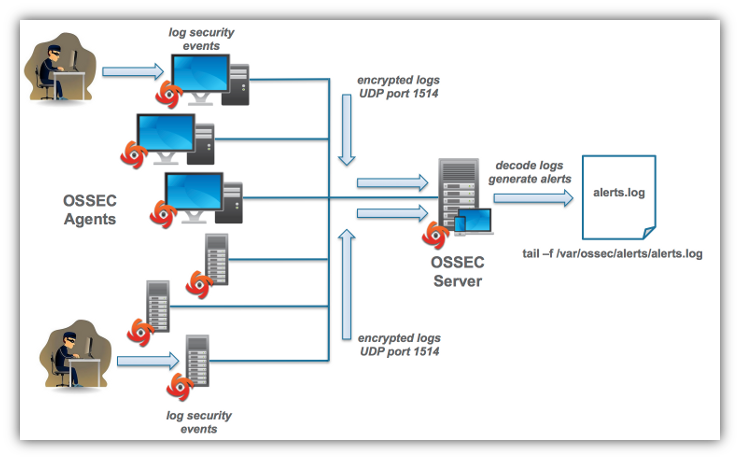
\includegraphics[width=6in,height=3in,keepaspectratio=true]{server-agent.png}
	\caption{Mô hình Server-agent trong OSSEC}
\end{figure}
	\begin{itemize}
	  \item Mô hình server-agent thích hợp khi cài đặt lên hệ thống có nhiều máy tính, ví
	như như trong 1 công ty, 1 phòng nghiên cứu, nhằm mục đích quản lý tập trung
	toàn bộ hệ thống. Mô hình này đòi hỏi thiết lập 1 máy tính đóng vai trò server, và các máy tính còn lại là các agent.
	\item Về phía server: Server sẽ có đầy đủ tính năng của OSSEC, như việc kiểm tra
	 toàn vẹn file, giám sát thanh ghi, phát hiện rootkit,... ngoài ra có thêm các
	 chức năng như thu thập log file, ghi file log cảnh báo, đặt luật cho toàn bộ hệ thống IDS.
	 \item Về phía agent:
Agent chỉ có các chức năng sau:
kiểm tra toàn vẹn file,
giám sát thanh ghi,
phát hiện rootkit,
active response.
Các chức năng như ghi file log cảnh báo, xem file log, thu thập syslog, đặt luật
đều được tập trung tại server.
\item Mô hình này cung cấp khả năng triển khai hệ thống an ninh để bảo vệ hệ thống
trên các máy tính và tập trung dữ liệu xử lý trên server, các agent sẽ loại bỏ
được công việc xử lý dữ liệu, và cơ chế tập trung về quy định và xử lý giúp quản
lý tốt hơn.   
	\end{itemize}
  
\section{Cách thức hoạt động trong OSSEC}
  \begin{figure}[h!]
	\centering 
	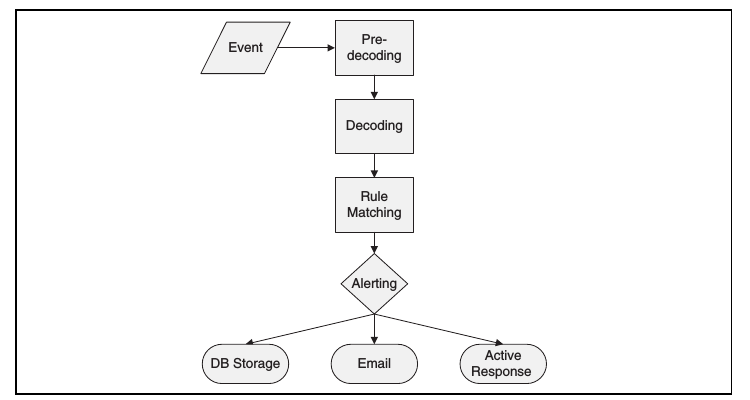
\includegraphics[width=6in,height=3in,keepaspectratio=true]{eventFlow.png}
	\caption{Cách thức hoạt động của OSSEC}
  \end{figure}
  
     \subsection{Nhận event}
     Event là những log file của các chương trình khi được thực thi, các
     chương trình trên máy tính khi thực thi đều tạo ra file log để ghi lại hành
     động.\\
     Chương trình OSSEC sẽ đọc tất cả các log file này mỗi khi chương
     trình khác thực thi. Từ file log này, OSSEC sẽ thực hiện công việc tiếp theo.
     \subsection{Rút trích dữ liệu}
     Tiến hành Decode và rút trích những thông tin liên quan từ event,
     phần decode được thực hiện thông qua 2 giai đoạn:\\
       \subsubsection{Predecoding}
       Rút trích các thông tin static từ event từ các trường
       quen thuộc và đơn giản, như ngày, giờ, log, hostname, tên chương trình.
       \begin{figure}[h!]
	\centering 
\fbox{	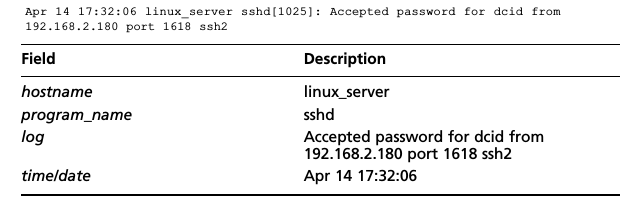
\includegraphics[width=6in,height=3in,keepaspectratio=true]{predecode_example.png}}
	\caption{Predecoder}
  \end{figure}\\
Predecoding hoạt động không dựa vào nguồn dữ liệu đầu vào của
         event. Vì tất cả các event đều sẽ có chung các thông tin đơn giản mà
         predecoding rút trích.\\\\
        Khi xử lý log: OSSEC sẽ chuẩn hóa các kiểu log khác nhau thành 1
         kiểu chuẩn do OSSEC định nghĩa, từ đó có thể viết các rules theo kiểu
         chuẩn này để rút trích được các thông tin cần thiết. Ngoài ra còn có
         thể định nghĩa rule để xét từng trường riêng với nhau: hostname hoặc
         program\_name.\\\\ 
         Ví dụ: Syslog ở hình trên và ASL ở hình dưới có log file hoàn toàn khác
         nhau, nhưng cũng có thể rút trích được theo các trường như decoder ở
         trên.
          \begin{figure}[h!]
	\centering 
\fbox{	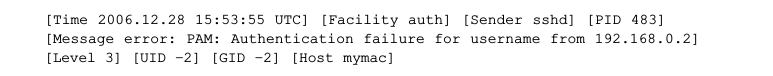
\includegraphics[width=6in,height=3in,keepaspectratio=true]{predoced_another_ASL.png}}
	\caption{Log của ASL}
  \end{figure}
  		\subsubsection{Decoding}
  		Đây là bộ phận quan trọng nhất trong quá trình hoạt động của OSSEC, các
  		thông tin quan trọng để xác định sự kiện được lấy ra trong quá trình
  		này.\\\\
  		Decoding rút
  		trích những thông tin mà phần predecoding chưa lấy được, như usernames hoặc địa chỉ IP nguồn, \ldots \\\\
  		Khác với predecoder, các thông tin do decoder rút trích khác nhau giữa các
  		event, do vậy mỗi 1 event đều có 1 decoder riêng, toàn bộ các decoder đều
  		được đặc tả trong file decoders.xml.\\\\
  	 Các trường có trong 1 decoder được miêu tả trong bảng dưới.
  	 \begin{table}[h]
  	 	\centering
		\begin{tabular}{|p{3cm}|p{10cm}|}
		
  			\hline
  			\textbf{Tag} & \textbf{Miêu tả}\\
		 \hline
  			program\_name & Thực thi decoder khi tên chương trình trong file log
  			trùng với program\_name\\
  			\hline
  			prematch & Thực thi decoder khi prematch trùng với bất kỳ phần nào trong
  			log\\
  			\hline
  			regex & Regular Expression để so sánh với log, rút trích những dữ liệu   			trùng
  			\\
  			\hline 
  			offset & Thuộc tính của regex. Để báo so sánh regex bắt đầu từ đâu, có 2
  			giá trị là after\_prematch và after\_parent\\
  			\hline
  			order & Thứ tự trong regex khi rút trích dữ liệu. Có thể là sự kiện
  			thường gặp (srcip, user, dstip, dstport, \dots)\\
  			\hline
  			parent & Decoder cha trước khi xét đến decoder này.\\
  			\hline  
  		\end{tabular}
  		\caption{Các trường trong decoder}
	\end{table}\\
	Với những trường này, decoder cung cấp các tính năng như so sánh theo tên
	chương trình (program\_name) hoặc so trùng thông tin (prematch). Ngoài ra
	decoder còn xếp sắp theo nhiều cấp trong mô hình cây giúp cho việc tạo decoder
	dễ dàng hơn, có tính kế thừa và mở rộng cao.\\\\
	 Dưới đây là 1 ví dụ về decoder của 1 đoạn log của ACL. Trong đoạn log sử dụng
  các tag \textless parent\textgreater{} để kế thừa decoder cha, \textless
  type\textgreater{} để xét định loại decoder, xác định tường để so sánh bằng
  \textless prematch\textgreater, sau đó xác định thông tin cần rút trích bằng \textless regex\textgreater{} và
  \textless order\textgreater.
	\begin{figure}[h!]
	\centering 
\fbox{	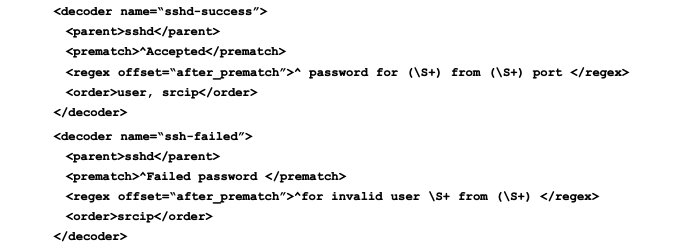
\includegraphics[width=6in,height=3in,keepaspectratio=true]{decoder_parent.png}}
	\caption{Decoder}
  \end{figure}
 
   \begin{figure}[h!]
	\centering 
\fbox{	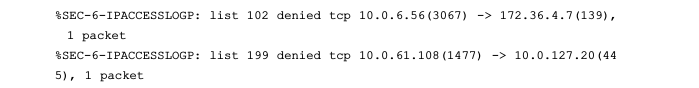
\includegraphics[width=6in,height=3in,keepaspectratio=true]{logACL.png}}
	\caption{Đoạn log của ACL}
	\end{figure}
	\begin{figure}[h!]
	\centering 
\fbox{	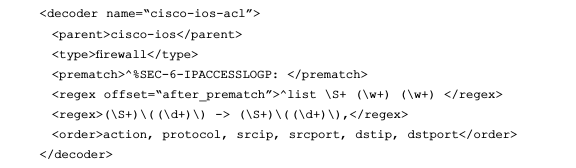
\includegraphics[width=6in,height=3in,keepaspectratio=true]{decoACL.png}}
	\caption{Decoder cho đoạn log ACL}
  \end{figure}
       \subsection{Rule matching}
        Sau khi rút trích được dữ liệu từ event, 1 cơ
       chế so sánh rules được gọi để xác định tính chất của event và quyết định điều khiển báo động.
\section{Về rules trong OSSEC}
Rules được định nghĩa trong các file xml riêng cho từng vấn đề (apache,
syslog, \dots), 1 file chứa nhiều rule.\\\\  
Mỗi rules được gán 1 ID cố
định và 1 mức độ (level) của rules đó.
  \subsection{ Về ID}
  \begin{itemize}
    \item Rules trong OSSEC có ID từ 00000 đến 50799, các rule được chia nhóm
    theo từng chức năng riêng, có các nhóm quan trọng như:
    \begin{itemize}
      \item 01000 - 01999: Rule cho syslog
      \item 05100 - 05299: Rule cho nhân hệ thống Linux, UNIX, BSD
      \item 30100 - 30999: Rule cho Apache HTTP server
      \item 31100 - 31199: Rule cho truy cập web 
      \item 50100 - 50299: Rule cho MySQL database
      \end{itemize}
      \item Ngoài ra, người dùng có thể tự định nghĩa rule có ID từ 100000 đến
      119999
      \item Khi sử dụng mô hình server-agent, các agent có thể có rules riêng
      cho bản thân, các rules này sẽ được viết vào trong file local\_rules.xml.
  \end{itemize}
  \subsection{Về mức}
  \begin{itemize}
    \item OSSEC gồm có 16 mức: 0 - 15, số mức cáng cao càng có độ cảnh báo cao.
    \item Mức 0 là mức đặc biệt, mang ý nghĩa là bỏ qua. Khi 1 rules được đánh
    giá là mức 0, event đó sẽ được bỏ qua và không xét tới nữa.
    \item Các luật trong OSSEC được lưu trữ theo cấu trúc cây, luật với mức cao
    được đánh giá trước, nhưng trước tiên phải xét luật với mức 0 vì đây là trường hợp đặc biệt, sẽ bỏ qua tất cả.
  \end{itemize}
  \subsection{Atomic rules}
  \begin{itemize}
    \item Là các luật chỉ xét riêng cho từng event riêng lẻ.
    \item Các tag chính trong rule:
    \begin{itemize}
      \item Tất cả các rule trong OSSEC đều được đặt trong tag \textless
      group\textgreater, \textless group\textgreater{} là tag để quản lý các
      loại rule có chung đặc điểm, mỗi group có tên để nêu lên đặc điểm của rule trong đó, như syslog, sshd, \dots
      \item Trong OSSEC cung cấp cơ chế kế thừa giữa các rules, 1 event sau khi
      được rút trích, thông tin đó sẽ được so sánh với rule cha, nếu trùng sẽ so
      sánh tiếp xuống rule con, như vậy sẽ tiết kiếm được chi phí so sánh khi
      không cần thiết phải so sánh hết với toàn bộ tập rule, và sẽ cung cấp khả
      năng để các rules mở rộng theo nhiều hướng từ 1 rules chính. Sử dụng thừa
      kế bằng cách thừa kế group chứa rule với tag \textless group\textgreater.
      \item Có các group lớn mà OSSEC đã định nghĩa sẵn, có thể sử dụng những
      group này làm group cha khi người dùng tự định nghĩa các rule.
      \begin{figure}[h!]
	\centering 
\fbox{	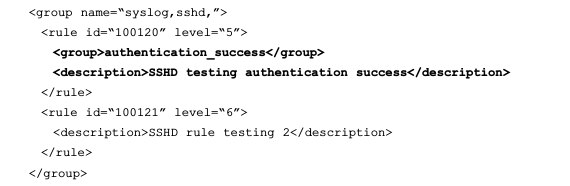
\includegraphics[width=6in,height=3in,keepaspectratio=true]{rule_subgroup.png}}
	\caption{Subgroup trong group}
  \end{figure}
      \item Sử dụng tag \textless decoded\_as\textgreater{}  để xác định decoder
      để decode event, rule được xác định decoder chỉ so sánh khi được decoder đó decode.
      \item Sử dụng tag \textless match\textgreater{}  để hỗ trợ cho tag \textless
      decoder\_as\textgreater, tag \textless match\textgreater{}  để so sánh trùng với nội dung mà decoder rút trích được. 
      \begin{figure}[h!]
	\centering 
\fbox{	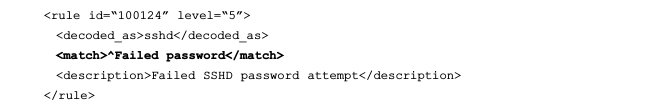
\includegraphics[width=6in,height=3in,keepaspectratio=true]{rule_match.png}}
	\caption{Tag match trong rule}
  \end{figure}
  	  \item Ngoài ra còn có các tag như \textless hostname\textgreater,
  	  \textless srcip\textgreater{}   để kiểm tra cụ thể theo yêu cầu như hostname hoặc srouce ip.
  	  \begin{figure}[h!]
	\centering 
\fbox{	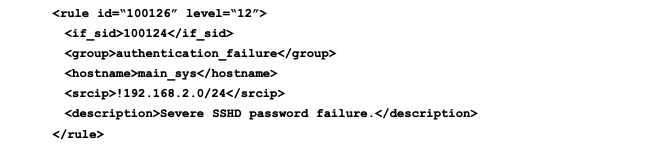
\includegraphics[width=6in,height=3in,keepaspectratio=true]{rule_scrip.png}}
	\caption{Tag scrip trong rule}
  \end{figure}
      \item Tag \textless time\textgreater{}  để kiểm tra về thời gian của event, để xác định chính
      xác hơn về quy định. Ví dụ như việc login vào server chỉ nên xảy ra trong thời gian làm việc, việc mọi sự đăng nhập ngoài giờ làm việc sẽ được cảnh báo ở mức cao hơn.
      \begin{figure}[h!]
	\centering 
\fbox{	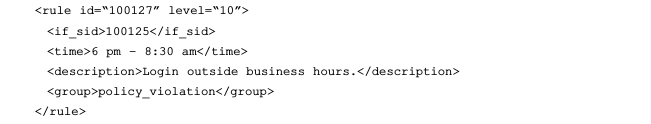
\includegraphics[width=6in,height=3in,keepaspectratio=true]{rule_time.png}}
	\caption{Tag time trong rule}
  \end{figure}
      \item Lưu ý là 1 sự kiện chỉ tạo ra 1 alert, rule được so sánh theo sơ đồ
      cây và node cuối cùng được so sánh trùng sẽ phát ra alert với mức của rule đó.
    \end{itemize}
  \end{itemize}
  \subsection{Composite rules}
  \begin{itemize}
    \item  Composite rules không xét có event riêng lẻ với nhau, mà so sánh
    event hiện tại với các event đã bắt được trước đó. Để các rule có để giữ được trạng thái, 1 rule phải có thêm hai thuộc tính sau:
    \begin{itemize}
      \item Frequency: để lấy tần số xuất hiện của event (event/pattern), tần số
      đủ lớn mới cảnh báo.
      \item Timeframe: xem xét lại thời gian từ event bây giờ tới thời điểm
      event trước đó  là bao nhiêu giây.
      \end{itemize}
      \begin{figure}[h!]
	\centering 
\fbox{	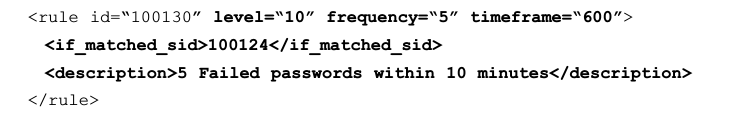
\includegraphics[width=6in,height=3in,keepaspectratio=true]{fre_time.png}}
	\caption{Tần số trong composite rule}
  \end{figure}
    \item Event được đếm tần số xuất hiện có thể dựa trên id \textless
    if\_match\_sid\textgreater, dựa trên group \textless
    if\_match\_group\textgreater, dựa trên regex \textless
    if\_match\_regex\textgreater.
    \item Ngoài ra có thể tăng độ chính xác và giảm lỗi bằng các tag so sánh
    cùng ip, port, hostname, program name.
     \begin{table}[h]
  	 	\centering
		\begin{tabular}{|p{3cm}|p{10cm}|}
		\hline
		\textbf{Tag} & \textbf{Miêu tả}\\
		 \hline
		 same\_source\_ip & Địa chỉ IP của Source phải giống nhau\\
		 \hline
		 same\_dest\_ip & Địa chỉ IP của Dest phải giống nhau\\
		 \hline
		 same\_src\_port & Địa chỉ Port của Source phải giống nhau\\
		 \hline
		 same\_dst\_port & Địa chỉ Port của Dest phải giống nhau\\
		 \hline
		 same\_location & Phải cùng 1 host hoặc agent\\
		 \hline
		 same\_user & Username được rút trích phải giống nhau\\
		 \hline
		 same\_id & ID được rút trích phải giống nhau\\
		 \hline
		\end{tabular}
		\caption{Các tag trong composite rule}
	  \end{table}
  \end{itemize}\vfill
\section{Cách thức cấu hình để OSSEC hoạt động}
Tất cả các cấu hình cơ bản cho OSSEC đều nằm trong file ossec.conf, file này
được viết bằng xml. File cấu trúc xml được chọn vì nhiều lý do: dễ đọc và dễ tìm
kiếm tới những phần cụ thể, cấu trúc kế thừa trong xml giúp cho việc xác định
nơi bắt đầu và kết thúc của từng phần cấu hình dễ dàng hơn, file xml có thể được
ghi 1 cách tự động từ chương trình cũng có thể dễ dàng thay đổi từ bất cứ 1 công
cụ đọc text nào.\\\\ 
Trong file ossec.conf có các tag lớn sau:
\begin{table}[h!]
  	 	\centering
		\begin{tabular}{|p{4cm}|p{9cm}|}
		\hline
		\textbf{Thành phần} & \textbf{Miêu tả}\\
		 \hline
		 \textless global\textgreater & Những cấu hình chung cho hệ thống trong mô
		 hình local hoặc là riêng server\\
		 \hline
		 \textless alerts\textgreater & Tùy chọn cho cảnh báo email và log\\
		 \hline
		 \textless email\_alerts\textgreater & Tùy chọn chi tiết cho cảnh báo email\\
		 \hline
		 \textless remote\textgreater & Cấu hình riêng cho các agent từ xa (chỉ áp
		 dụng cho server)\\
		 \hline
		 \textless database\_output\textgreater & Tùy chọn cho việc ghi log vào trong
		 database\\
		 \hline
		 \textless rules\textgreater & Liệt kê tất cả những file rule được sử dụng\\
		 \hline
		 \textless client\textgreater & Cấu hình liên quan đến agent\\
		 \hline
		 \textless localfile\textgreater & Cấu hình cho việc giám sát log file\\
		 \hline
		 \textless syscheck\textgreater & Cấu hình cho việc kiểm tra tính toàn vẹn\\
		 \hline
		 \textless rootcheck\textgreater & Cấu hình cho việc kiểm tra rootkit và điều
		 lệ\\
		 \hline
		 \textless command\textgreater & Cấu hình cho active response\\
		 \hline
		 \textless active-response\textgreater & Cấu hình nâng cao cho active
		 response\\
		 \hline
		 \end{tabular}
		 \caption{Các thành phần trong file ossec.conf}
\end{table}\\
  Cách thức cấu hình cụ thể sẽ được trình bày theo từng module riêng trong
mục các module trong OSSEC.
\section{Các module trong OSSEC}
  \subsection{Log alert và email alert}
  \begin{itemize}
    \item Đây là module cơ bản và quan trọng nhất trong OSSEC, cần điều chỉnh module này phù hợp với hệ thống cài đặt để tối ưu theo ý muốn người sử dụng.
    \item Theo mặc định, khi event tạo ra alert với mức từ 1 đến 15 đều được OSSEC ghi vào trong log file. Các sự kiện trên mức 7 sẽ được OSSEC gửi email để alert cho admin.
    \item Để thay đổi mức cảnh báo này, có thể sử dụng 2 trường trong tag
    \textless alert\textgreater, đó là \textless log\_alert\_level\textgreater{} và
    \textless email\_alert\_level\textgreater.
    \begin{figure}[h!]
	\centering 
\fbox{	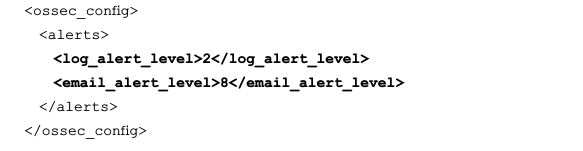
\includegraphics[width=6in,height=3in,keepaspectratio=true]{mail_alert.png}}
	\caption{Cấu hình mức cảnh báo email của OSSEC}
  \end{figure}
     \item Email alert là 1 tính năng rất hữu dụng trong OSSEC, vì nó cung cấp
     khả năng phản ứng nhanh chóng với các cảnh báo.
     \item Để cấu hình tính năng email alert, sử dụng các tag trong tag
     \textless global\textgreater.
     \begin{figure}[h!]
	\centering 
\fbox{	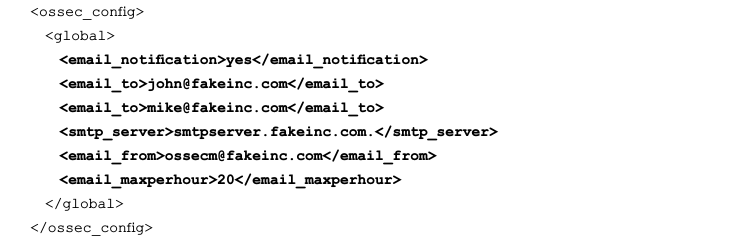
\includegraphics[width=6in,height=3in,keepaspectratio=true]{email_name.png}}
	\caption{Cấu hình email cảnh báo trong OSSEC}
  \end{figure}
  \item Ngoài ra còn có các tính năng hỗ trợ thêm trong tag
  \textless email\_alerts\textgreater:
  \begin{itemize}
    \item Tag \textless group\textgreater: xác định nhóm alert của chương trình
    nào sẽ gửi email đến địa chỉ trên.
    \item Tag \textless level\textgreater: xác định mức của cảnh báo để gửi
    email.
    \item Tag \textless format\textgreater: xác định cách thức gửi cảnh báo. Sms
    để gửi cảnh báo bằng tin nhắn.
    \item Tag \textless event\_location\textgreater: xác định chỉ những cảnh báo
    đến từ các agent nào mới gửi cảnh báo.
    \end{itemize}
  \end{itemize}
  \subsection{Xác định file rules}
  Trong OSSEC cho phép include các file rules cần thiết để xác định rule nào
  được kiểm tra, các file rule đều nằm trong đường dẫn ossec/rules. File rules
  được xác định phải nằm trong tag \textless include\textgreater.
  \begin{figure}[h!]
	\centering 
\fbox{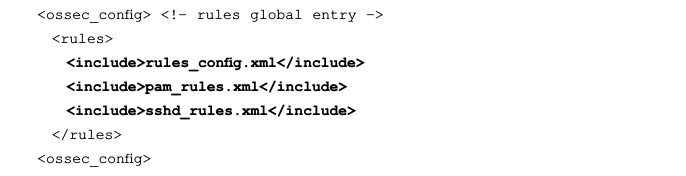
\includegraphics[width=6in,height=3in,keepaspectratio=true]{conf_rule.png}}
	\caption{Liệt kê file rule trong ossec.conf}
  \end{figure}
  \subsection{Kiểm tra toàn vẹn hệ thống}
  \begin{itemize}
    \item Phần cơ bản và quan trọng nhất trong 1 HIDS, cơ bản là kiểm tra
    checksum của file so với checksum bản file tốt để xem file có bị thay đổi hay không.
    \item Kiểm tra toàn vẹn file có thể giúp chống lại các loại trojans, phần
    mềm độc hại có khả năng thay đổi mã chương trình.
    \item Trong OSSEC việc kiểm tra tính toàn vẹn thông qua 3 tag chính trong
    tag \textless syscheck\textgreater:
    \begin{itemize}
      \item Tag \textless directory\textgreater: cung cấp cơ chế để xác định
      folder được kiểm tra toàn vẹn.
      \item Tag \textless ignore\textgreater: xác định file, folder có thể bỏ qua trong
      lúc kiểm tra.
      \item Tag \textless frequency\textgreater: xác định tần số kiểm tra.
    \end{itemize}
    \begin{figure}[h!]
	\centering 
	\fbox{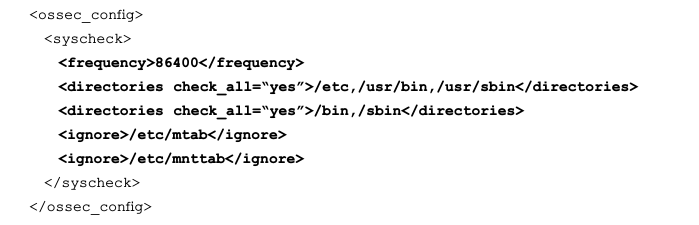
\includegraphics[width=6in,height=3in,keepaspectratio=true]{syscheck.png}}
	\caption{Cấu hình kiểm tra tính toàn vẹn trong ossec.conf}
  \end{figure}
    \item Tạo rules mới nên sử dụng \textless
    if\_group\textgreater syscheck\textless /if\_group\textgreater{} để bao hàm
    group syscheck của OSSEC.
  \end{itemize}
  \subsection{Kiểm tra và phát hiện rootkit}
  \begin{itemize}
    \item OSSEC chỉ có thể kiểm tra rootkit trên hệ điều hành Linux, Unix, và BSD, bên cạnh đó cũng cung cấp khả năng kiểm tra về điều lệ (policy) trên hệ thống Windows, Linux, Unix và BSD.
    \item OSSEC kiểm tra rootkit mức ứng dụng thông qua dấu hiệu và rootkit mức hệ thống thông qua so sánh system call. Ngoài ra còn cung cấp khả năng kiểm tra theo kiểu bất thường (anomaly) để có thể đạt yêu cầu người sử dụng.
    \item Trong mô hình server-agent, việc cấu hình kiểm tra điều lệ (policy) và kiểm tra rootkit được hiện thực trên server và đưa xuống agent.
  \end{itemize}
 \section{Giao diện web OSSEC - OSSEC WUI}
 \subsection{Phần giới thiệu}
 OSSEC HIDS Web User Interface (WUI) cung cấp một giao diện dựa trên web mà thực
 hiện các phân tích thống kê và mối tương quan của dữ liệu thay vì sử dụng các
 thao tác dòng lệnh (command line) để thực hiện.\\\
  Các trang điều khiển chính
 mang lại cho chúng ta một cái nhìn tổng quát vào những gì đang xảy ra khi triển
 khai OSSEC HIDS. Một công cụ tìm kiếm mạnh mẽ có sẵn để theo dõi các sự kiện 
 mà OSSEC HIDS thu thập được và cảnh báo. Tất cả những tập tin bị thay đổi tính
 toàn vẹn được ghi lại, và một giao diện thân thiện cho phép xem các thay đổi
 tập tin theo thời gian. Cuối cùng, một thống kê hữu ích cho phép tổng hợp tất
 cả các sự kiện và cảnh báo được thu thập để cung một cái nhìn thống kê những gì
 đang xảy ra trên mạng của máy tính chúng ta.
 \subsection{Phần cài đặt}
 Các WUI được hỗ trợ trên các hệ điều hành Linux, Unix, và hệ điều hành BSD với
 điều kiện hệ điều hành có khả năng chạy:
 \begin{itemize}
   \item OSSEC HIDS phiên bản 0,9-3 và mới hơn.
   \item Apache HTTP Server là phần mềm để thực hiện HTTP Web Server.
   \item PHP 4.1 và mới hơn:  PHP là một sử dụng rộng rãi, ngôn ngữ general –
   purpose đặc biệt phù hợp để phát triển Web và có thể được nhúng vào HTML.
 \end{itemize}
 \subsection{Thành phần}
Web User Interface có nhiều tab, mỗi trong số đó phục vụ một mục đích, chức năng
cụ thể.
\begin{itemize}
  \item Main: Giao diện điều khiển chính.
  \item Search: Cho phép bạn tìm kiếm thông qua thu thập HIDS OSSEC cảnh báo.
  \item Integrity Checking:  Cho phép bạn tìm kiếm thông qua thu thập từ cảnh
  báo syscheck OSSEC HIDS.
  \item Stats: Hiển thị thống kê về thu OSSEC HIDS cảnh báo.
  \item About:  Hiển thị cấp giấy phép và thông tin bản quyền về các HIDS OSSEC
  và các WUI.
\end{itemize}
\begin{figure}[h!]
	\centering 
	\fbox{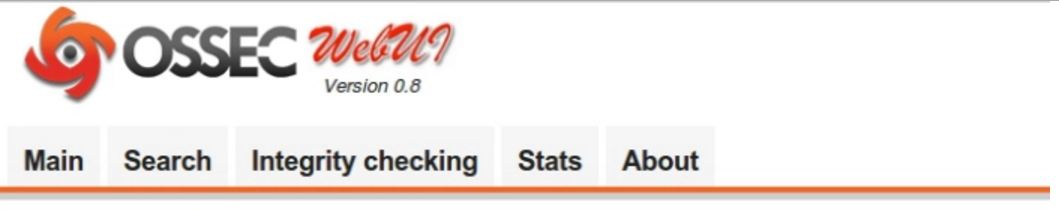
\includegraphics[width=6in,height=3in,keepaspectratio=true]{WUInav.jpg}}
	\caption{Thanh công cụ quản lí WUI của OSSEC}
  \end{figure}
  \begin{enumerate}
    \item Main\\
    Main là giao diện chính của WUI cho phép người dùng có thông tin hợp lệ của
    WUI để xem được những thông tin diễn ra trong việc triển khai OSSEC HIDS.
    Gồm có ba phần chi tiết với nhiệm vụ cụ thể là: Available agents, Latest
    modified files, Latest events.
    \begin{itemize}
      \item Available Agents\\
      Tất cả các cấu hình được hiển thị có sẵn trên tab Main. Các tên agent và địa chỉ IP liên kết được hiển thị cho từng agent. Nếu agent không hoạt động hoặc không thể kết nối đến máy chủ OSSEC HIDS, inactive được hiển thị bên cạnh tên agent.
Nhấp chuột vào các agent cho bạn thông tin chi tiết hơn về máy tính mà
OSSEC HIDS agent được cài đặt.
	  \begin{figure}[h!]
	\centering 
	\fbox{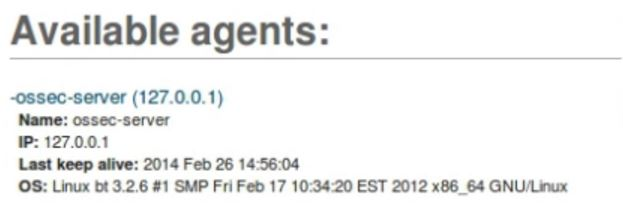
\includegraphics[width=6in,height=3in,keepaspectratio=true]{WUI2.jpg}}
	\caption{Giao diện hiển thị agent hiện có}
  \end{figure}
  \item Latest Modified Files
  \begin{itemize}
    \item Các tập tin mới được sửa đổi (Latest Modified Files) cho thấy một
    danh sách đầy đủ của các tập tin thay đổi mới nhất cho tất cả các agent. Mỗi tập tin sửa đổi được liệt kê theo ngày mà dịch vụ syscheck Báo cáo thay đổi để các máy chủ OSSEC HIDS. Như đã thấy trong hình 7.2, khi bạn nhấn vào tập tin sửa đổi,chi tiết cho các tập tin được hiển thị.
    \item Số lượng các tập tin sửa đổi phụ thuộc vào số lượng agent bạn có cấu
    hình. Điều này được xác định bởi agent\_count + 4 phương trình, agent\_count
    là số lượng agent bạn đã cấu hình. Nếu bạn có 10 agent, nó sẽ chỉ hiển thị
    14 tập tin sửa đổi cuối cùng. Tương tự như vậy, nếu bạn chỉ có một agent, nó
    sẽ chỉ hiển thị năm tập tin sửa đổi cuối cùng. Phương trình agent\_count + 4
    được đặt ra để đảm bảo rằng các giao diện người dùng vẫn duy trì cấu trúc như agent thêm vào được cấu hình.
    \end{itemize}
    \item Latest Events\\
    The Latest events đưa ra các sự kiện mới nhất mà được báo cáo bởi OSSEC HIDS
    agents cho OSSEC HIDS server. Bao gồm một số thông tin cơ bản như: Thời
    gian, chỉ số rule, cấp độ, địa chỉ IP agent, miêu tả, \ldots
   \end{itemize}
   \item Search\\
   Các WUI cung cấp một công cụ tìm kiếm cho phép bạn lọc các tiêu chí cụ thể và
   xem kết quả tìm kiếm trong thời gian thực hoặc thực hiện các phân tích lịch sử trên dữ liệu sự kiện được lưu trữ. Tab tìm kiếm được chia thành ba phần, mỗi phần có một mục đích cụ thể: Tùy chọn tìm kiếm thông báo (Alert search options), kết quả (results) và danh sách thông báo (Alert list)
   \begin{itemize}
     \item Alert Search Options\\
     Cho phép ta xác định các tiêu chí tìm kiếm cảnh báo mà bạn muốn xem.
     Đồng thời nó còn cho phép chúng ta chọn một ngày và phạm vi thời gian cho các cảnh báo được lưu trữ mà chúng ta cần. Nếu chúng ta muốn xem cảnh báo trong thời gian thực thì ta chọn Real time monitoring và chọn các tiêu chí phù hợp. Một số tiêu chí như:
     \begin{itemize}
       \item Minimum level: Đưa ra mức cảnh báo thấp nhất để lọc. Mặc định là
       tất cả (All) và phạm vi là từ 2 đến 15.
       \item Pattern: Chỉ định một mô hình phù hợp để các cảnh báo được tạo ra.
       Mô hình đơn giản matching và công thức Perl regular có thể được sử dụng.
       \item Srcip: Lọc trên một IP nguồn cụ thể trong thông báo được tạo ra.
       \item Location: Bộ lọc trên một OSSEC HIDS agent cụ thể.
     \end{itemize}
     Khi đã hoàn thành việc cấu hình tiêu chuẩn các tiêu chí của bộ lọc tìm kiếm
     cảnh báo, chúng ta phải bấm nút Tìm kiếm (Search) để lấy hồ sơ cảnh báo.
     \item Results\\
     Phần kết quả cho thấy các kết quả truy vấn thông báo dựa trên các bộ lọc
     thiết lập trong Alert Search Options. Ở phía trên của phần kết quả là tổng
     số cảnh báo tìm thấy phù hợp với tiêu chí tìm kiếm. Thông tin sau đó được
     hiển thị trong ba nhóm riêng biệt cho phép chúng ta xem các phân tích kết quả bởi : Mức độ nghiêm trọng (Severity), Rule và IP nguồn ( Src IP).\\
     Trong mỗi nhóm, chúng ta có thể tùy chọn để hiển thị hoặc ẩn các thông báo
     của các loại được chọn. Nhấp vào liên kết màu đỏ bên cạnh các mục nhập bộ
     lọc và có thể bao gồm các mục khác trong bộ lọc.\\
     Ở dưới phần kết quả là các đường dẫn đến các sự kiện đầu tiên và cuối cùng
     nhìn thấy dựa trên bộ lọc cảnh báo hiện tại. Hai liên kết hiển thị ngày tháng và thời gian đóng dấu cho mỗi sự kiện.
     \item Alert List\\
     Danh sách cảnh báo sẽ hiển thị kết quả tìm kiếm với các bộ lọc được xác
     định trong Alert Search Options và phần Result.
   \end{itemize}
   \item Integrity Checking\\
   Phần kiểm tra tính toàn vẹn cung cấp hai tính năng rất quan trọng của WUI:
   một danh sách các tập tin bị sửa đổi của tất cả các agent, và một phương pháp
   dump toàn bộ syscheck cơ sở dữ liệu cho một agent cụ thể.\\
   \textbf{Latest Modified Files (cho tất cả Agents):}\\ 
Phần tập tin sửa đổi mới nhất cho thấy một danh sách đầy đủ của các tập tin bị
thay đổi mới nhất cho tất cả các agent. Mỗi tập tin sửa đổi được liệt kê theo
ngày mà các dịch vụ syscheck báo thay đổi cho máy chủ OSSEC HIDS.\\
	\textbf{Dump Database}\\
	Kiểm tra tính toàn vẹn cho phép bạn cấu hình một agent, và dump toàn bộ nội
	dung của cơ sở dữ liệu syscheck cho agent đó. Dưới phần Latest Modified Files,
	phần Integrity Checking database cung cấp một danh sách hoàn chỉnh của tất cả
	các tập tin hoặc các khóa registry của Windows mà dịch vụ syscheck đã thông báo
	một sự thay đổi tính toàn vẹn. Một vài thông số như : Tên tập tin, mã hash (MD5 hay SHA-1), kích thước tập tin.
	\item Stats\\
	WUI có một công cụ báo cáo thống kê mạnh mẽ cho phép nhanh chóng hiển thị
của các cảnh báo của bạn OSSEC, thay đổi syscheck, và cảnh báo tường lửa cho bất
kỳ ngày, tháng, hoặc năm. Điều này mang đến khả năng chọn một điểm và hiển thị
các thông báo liên quan được  tạo ra bởi các agent và thu thập bởi máy chủ.\\
    WUI được chia thành ba phần báo cáo chính, mỗi phần cung cấp một tổng hợp
    thu thập cảnh báo khác nhau: giá trị tổng hợp bởi mức độ nghiêm trọng, giá
    trị tổng hợp theo rule, tổng giá trị mỗi giờ.
    \begin{itemize}
      \item Giá trị tổng hợp bởi mức độ nghiêm trọng (Aggregate values by
      severity) cho bạn thấy tổng số các cảnh báo được chia nhỏ bởi mức độ nghiêm trọng của các cảnh báo.
      \item Giá trị tổng hợp theo rule (Aggregate Values by Rule ) cho thấy tổng
      số các cảnh báo được chia nhỏ bởi các rule mà tạo ra các cảnh báo.
      \item Tổng giá trị mỗi giờ (Total Values per Hour) cho thấy tổng số các
      cảnh báo được chia nhỏ theo giờ mà các cảnh báo đã báo cáo với OSSEC HIDS
    \end{itemize}
	\item About\\
	Phần giới thiệu của WUI cung cấp bản quyền và thông tin giấy phép cho WUI và
	các OSSEC HIDS. Giấy phép chỉ ra rằng OSSEC HIDS là phần mềm miễn phí và rằng nó có thể phân phối hoặc sửa đổi theo các điều khoản của GNU General Public License (phiên bản 3). Giấy phép này như được xuất bản bởi Free Software Foundation.
  \end{enumerate}
